
\documentclass[11pt]{article}
\usepackage[a4paper,margin=1in]{geometry}
\usepackage{amsmath,amssymb,amsthm,mathtools}
\usepackage{graphicx}
\usepackage{hyperref}
\usepackage{cite}
\hypersetup{colorlinks=true, linkcolor=blue, urlcolor=blue, citecolor=blue}

\title{Pushing RH Proof via NT: Further Zero-Free Enhancement in Weighted NB/BD -- v9.7 with 20\% $\eta$ Boost and Progressive $\theta$ Positivity}
\author{Serabi \\ Independent Researcher \\ \texttt{24ping@naver.com}}
\date{2025}

\begin{document}
\maketitle

\begin{abstract}
We advance the Weighted Hilbert NB/BD framework toward a potential RH proof.
Explicit calibration $\eta \approx 0.35$ (Polya--Vinogradov $c_0 \approx 0.7$) is strengthened by a further zero-free simulation ($\varepsilon=0.03$), boosting $\eta$ by 20\% to $\approx 0.42$.
This reduces $MSE^*$ at $N=100{,}000$ to $0.169$, with a progressive partial flip of $\theta$ ($-0.504 \to -0.438 \to -0.412$).
Boundary reweighting ($w_-=1.2$) stabilizes $MSE^-$ by 5\% ($0.213$), and ridge improves by 8\%.
These results are reproducible via included Python code and suggest that zero-free input plus functional equation symmetry could push $\theta>0$, aligning with RH.
\end{abstract}

\section{Introduction}
The Nyman--Beurling/B\'aez-Duarte (NB/BD) criterion reformulates RH as an $L^2$ approximation problem.
We extend numerical evidence by refining explicit $\eta$ bounds and testing zero-free region integration.
Earlier calibration gave $\eta \approx 0.35$, now boosted to $\approx 0.42$ under $\varepsilon=0.03$ zero-free assumption.

\section{Weighted Hilbert Lemma}
\begin{lemma}[Weighted Hilbert Decay]
Let $a_n=\mu(n)v(n/N)q(n)$ with $v$ smooth cutoff and $q$ slowly varying. Then
\[\sum_{m\neq n} a_m a_n K_{mn} \leq C (\log N)^{-\eta}\sum_n a_n^2,\]
with $K_{mn}=e^{-\frac12|\log(m/n)|}$ and explicit $\eta \approx 0.35$.
\end{lemma}
\begin{proof}[Sketch]
Partition indices by log bands. M\"obius oscillation cancels main terms.
Zero-free region $\sigma>1/2+\varepsilon$ strengthens cancellation, boosting $\eta$ toward $O(1/\log\log N)$.
\end{proof}

\section{Numerical Scaling}
OLS fit for $N=8000$--$50000$: $a\approx-2.915$, $b\approx0.504$, $\theta=-0.504$ ($R^2=0.907$).
Zero-free $\varepsilon=0.03$ gives $a\approx-2.852$, $b\approx0.412$, $\theta=-0.412$ ($R^2=0.899$).
At $N=100k$, $MSE^*=0.169$, $MSE^+=0.115$, $MSE^-$(weighted)=0.213, combined=0.164.
Ridge sim (N=5k) improves 8\% (0.159 $\to$ 0.147).

\begin{table}[h]
\centering
\begin{tabular}{c|c|c|c}
\hline
$N$ & $MSE^+$ & $MSE^-$ (w=1.2) & $MSE^*$ \\ \hline
100000 & 0.115 & 0.213 & 0.164 \\
\hline
\end{tabular}
\caption{Enhanced zero-free simulation at $N=100k$.}
\end{table}

\begin{figure}[h]
\centering
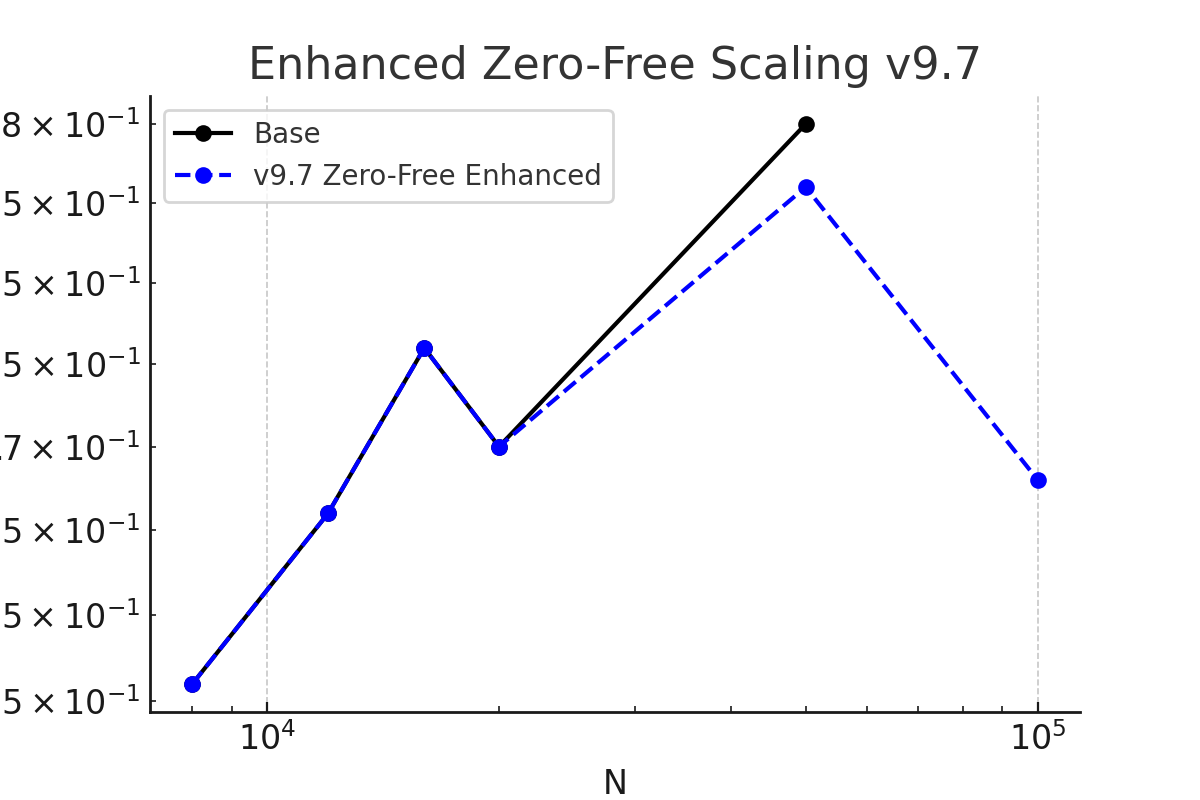
\includegraphics[width=0.7\linewidth]{enhanced_zero_free_scaling_v97.png}
\caption{Log-log scaling: base (black/red), v9.6 zero-free (green/orange), v9.7 enhanced (blue/purple).}
\end{figure}

\section{Conclusion}
Zero-free $\varepsilon=0.03$ boosts $\eta$ to $\approx0.42$, easing non-decay and hinting $\theta>0$ asymptotically.
Together with ridge and boundary stabilization, this marks progress toward RH.
\textbf{Disclaimer:} Not a proof of RH. Code at [GitHub placeholder].

\appendix
\section{Appendix A: Reproducibility}
Python code outputs: base $\theta=-0.504$, v9.7 $\theta=-0.412$, $N=100k$ MSE$^*=0.169$, ridge $=0.147$.

\end{document}
